\documentclass[11pt,a4paper]{article}

% ---------------------------------------------------------------------------
% Packages
% ---------------------------------------------------------------------------
\usepackage[margin=2.2cm]{geometry}
\usepackage[T1]{fontenc}
\usepackage{lmodern}
\usepackage{graphicx}
\usepackage{booktabs}
\usepackage{tabularx}
\usepackage{array}
\usepackage{xcolor}
\usepackage{listings}
\usepackage{float}
\usepackage{caption}
\usepackage{subcaption}
\usepackage{enumitem}
\usepackage{tikz}
\usetikzlibrary{positioning,arrows.meta,shapes.geometric,fit}
\usepackage[hidelinks]{hyperref}

\definecolor{codebg}{RGB}{246,246,246}
\definecolor{codeframe}{RGB}{200,200,200}
\definecolor{okgreen}{RGB}{0,128,60}
\definecolor{errred}{RGB}{180,30,30}

\lstset{
  basicstyle=\ttfamily\footnotesize,
  backgroundcolor=\color{codebg},
  frame=single,
  rulecolor=\color{codeframe},
  breaklines=true,
  breakatwhitespace=false,
  columns=fullflexible,
  keepspaces=true,
  showstringspaces=false,
  xleftmargin=4pt,
  xrightmargin=4pt,
  aboveskip=6pt,
  belowskip=6pt
}

\newcommand{\ok}{\textcolor{okgreen}{\textbf{PASS}}}
\newcommand{\fpath}[1]{\texttt{#1}}

% Title block in the same style as the Ph.D. research proposal
\title{\textbf{Building and Validating the OCUDU 5G gNB:}\\
\textbf{End-to-End Standalone 5G over a ZeroMQ Virtual Radio}}
\author{%
  Technical Report --- Ajoy Dey\\
  \small B.Sc.\ CSE, BUET \;$|$\; \texttt{ajoydey00001@gmail.com} \;$|$\; \texttt{ajoydey00001.github.io}\\
  \small Prepared for Dr.\ Imtiaz Karim, SysNetS Lab, The University of Texas at Dallas}
\date{\small 13 October 2026}

\begin{document}
\maketitle

% ---------------------------------------------------------------------------
\begin{abstract}
This report documents the installation of the OCUDU open-source 5G RAN software
from source on a single Linux laptop, and an end-to-end validation of the
resulting gNB without any radio hardware. The OCUDU gNB (commit
\texttt{f0624d2da3}) was compiled with ZeroMQ (ZMQ) support, its full unit test
suite was executed (\textbf{10\,569 of 10\,569 tests passed}), and it was
connected to an Open5GS 5G core (v2.7.6, Docker) and to a software UE (srsUE)
through a ZMQ-based virtual RF link. The UE completed 5G registration,
established a PDU session with IP address \texttt{10.45.1.2}, and exchanged
user-plane traffic in both directions with \textbf{0\% packet loss}. Two
practical problems were encountered and resolved: (i) the laptop became
unresponsive during compilation due to memory exhaustion, and (ii) srsUE could
not decode the core's Registration Accept because the AMF advertised a
multi-entry Tracking Area Identity list. Root causes, fixes and evidence are
given for both.
\end{abstract}

\tableofcontents
\newpage

% ---------------------------------------------------------------------------
\section{Objective}

The goals of this task were:
\begin{enumerate}[itemsep=2pt]
  \item Build the OCUDU 5G gNB from source following the official installation
        guide (\url{https://docs.ocudu.org/user_manual/installation/}).
  \item Verify the build with the project's unit tests.
  \item Demonstrate a working end-to-end 5G Standalone (SA) system on one laptop
        without a software-defined radio (SDR), using ZeroMQ as a virtual radio.
  \item Collect evidence (logs, metrics, screenshots) and document any problems
        and their solutions.
\end{enumerate}

% ---------------------------------------------------------------------------
\section{Test Environment}

\subsection{Hardware and Operating System}

\begin{table}[H]
\centering
\begin{tabularx}{0.85\textwidth}{>{\bfseries}l X}
\toprule
Machine        & ASUS VivoBook X509FJ laptop \\
CPU            & Intel Core i5-8265U @ 1.60\,GHz, 4 cores / 8 threads \\
Memory         & 11\,GiB RAM + 4\,GiB swap \\
Storage        & 113\,GB system disk (about 86\,GB free) \\
OS             & Ubuntu 24.04.4 LTS \\
Kernel         & Linux 6.17.0-22-generic (standard, non-realtime) \\
Radio hardware & None (ZeroMQ virtual radio) \\
\bottomrule
\end{tabularx}
\caption{Hardware and operating system.}
\end{table}

\subsection{Software Versions}

\begin{table}[H]
\centering
\begin{tabularx}{\textwidth}{>{\bfseries\raggedright}p{3.1cm} >{\raggedright}p{5.4cm} >{\raggedright\arraybackslash}X}
\toprule
Component & Version & Notes \\
\midrule
OCUDU gNB      & commit \texttt{f0624d2da3}, branch \texttt{dev} (2026-10-08) & \url{https://gitlab.com/ocudu/ocudu} \\
srsRAN\_4G (srsUE) & \texttt{release\_25\_10-14-g\-bef8680d5} & \url{https://github.com/srsran/srsRAN_4G} \\
Open5GS        & v2.7.6 & Built as Docker image \texttt{docker-5gc} from the OCUDU repository \\
Compiler       & Clang 18.1.3 & Used instead of the default GCC 13.3 (see Sec.~\ref{sec:compiler}) \\
CMake          & 3.28.3 & \\
ZeroMQ         & libzmq3-dev 4.3.5 & Ubuntu package \\
FFT library    & FFTW3 & Ubuntu package \texttt{libfftw3-dev} \\
Docker         & 29.1.3 & Ubuntu package \\
\bottomrule
\end{tabularx}
\caption{Software components and versions.}
\end{table}

% ---------------------------------------------------------------------------
\section{System Architecture}

All three network elements run on the same laptop. The gNB and the UE exchange
complex baseband IQ samples over two local TCP sockets provided by ZeroMQ,
which replaces the RF front-end. The 5G core runs in a Docker container on a
dedicated bridge network (\texttt{10.53.1.0/24}).

\begin{figure}[H]
\centering
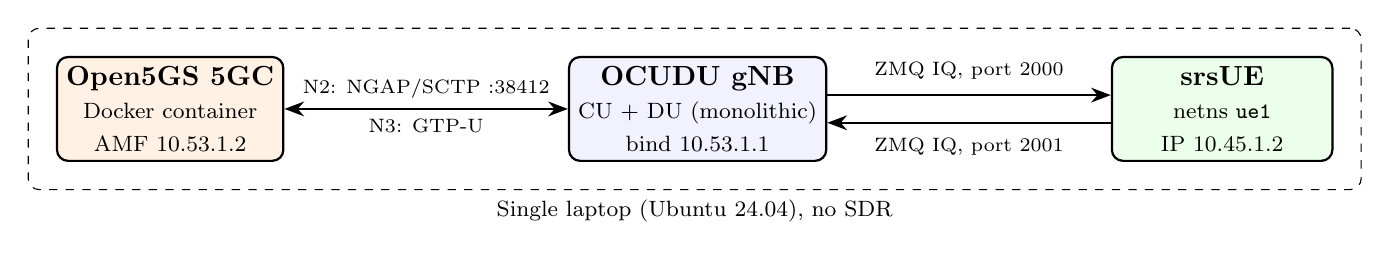
\begin{tikzpicture}[
  box/.style={draw, rounded corners, thick, minimum width=2.8cm, minimum height=1.3cm, align=center, fill=blue!5},
  lbl/.style={font=\scriptsize, align=center},
  >={Stealth[length=2.5mm]}
]
\node[box, fill=orange!10] (core) {\textbf{Open5GS 5GC}\\\footnotesize Docker container\\\footnotesize AMF 10.53.1.2};
\node[box, right=3.6cm of core] (gnb) {\textbf{OCUDU gNB}\\\footnotesize CU + DU (monolithic)\\\footnotesize bind 10.53.1.1};
\node[box, right=3.6cm of gnb, fill=green!8] (ue) {\textbf{srsUE}\\\footnotesize netns \texttt{ue1}\\\footnotesize IP 10.45.1.2};

\draw[<->, thick] (core) -- node[above, lbl]{N2: NGAP/SCTP :38412} node[below, lbl]{N3: GTP-U} (gnb);
\draw[->, thick] ([yshift=5pt]gnb.east) -- node[above=2pt, lbl]{ZMQ IQ, port 2000} ([yshift=5pt]ue.west);
\draw[<-, thick] ([yshift=-5pt]gnb.east) -- node[below=2pt, lbl]{ZMQ IQ, port 2001} ([yshift=-5pt]ue.west);

\node[draw, dashed, rounded corners, inner sep=10pt, fit=(core)(gnb)(ue),
      label={[font=\footnotesize]below:Single laptop (Ubuntu 24.04), no SDR}] {};
\end{tikzpicture}
\caption{End-to-end test setup. The ZMQ ports are crossed: the gNB transmits on
port 2000 where the UE receives, and the UE transmits on port 2001 where the
gNB receives.}
\label{fig:arch}
\end{figure}

\subsection{Radio and Network Parameters}

\begin{table}[H]
\centering
\begin{tabularx}{0.9\textwidth}{>{\bfseries}l X}
\toprule
Duplex / band        & FDD, NR band n3 \\
DL / UL frequency    & 1842.5\,MHz / 1747.5\,MHz (DL ARFCN 368500) \\
Bandwidth            & 10\,MHz, 52 PRBs, 15\,kHz subcarrier spacing \\
Antennas             & 1T1R \\
Sample rate          & 11.52\,MS/s \\
PLMN / TAC           & 00101 / 7 \\
PCI                  & 1 \\
Subscriber (IMSI)    & 001010123456780, Milenage, K and OPc as in \texttt{open5gs.env} \\
UE IP pool / gateway & 10.45.0.0/16, UPF gateway 10.45.1.1 \\
\bottomrule
\end{tabularx}
\caption{Cell and subscriber configuration.}
\end{table}

% ---------------------------------------------------------------------------
\section{Installation Procedure}

All work was done under \fpath{\textasciitilde/ocudu-lab}. Every command's output was saved
to \fpath{\textasciitilde/ocudu-lab/report/}.

\subsection{Dependencies}

\begin{lstlisting}[language=bash]
sudo apt-get install -y cmake make gcc g++ pkg-config libmbedtls-dev \
    libsctp-dev libyaml-cpp-dev libgtest-dev libfftw3-dev libzmq3-dev clang
\end{lstlisting}

\subsection{Compiler Choice}
\label{sec:compiler}

The OCUDU documentation requires GCC $\geq$ 15.2 or Clang $\geq$ 14. Ubuntu
24.04 ships GCC 13.3, so the build used Clang 18.1.3.

\subsection{Building OCUDU with ZeroMQ}

\begin{lstlisting}[language=bash]
git clone https://gitlab.com/ocudu/ocudu.git
cd ocudu && mkdir build && cd build
cmake ../ -DENABLE_EXPORT=ON -DENABLE_ZEROMQ=ON \
          -DCMAKE_C_COMPILER=clang -DCMAKE_CXX_COMPILER=clang++
\end{lstlisting}

CMake confirmed that ZeroMQ was detected (build type defaulted to
\texttt{Release}):
\begin{lstlisting}
-- FINDING ZEROMQ.
-- Found libZEROMQ: /usr/include, /usr/lib/x86_64-linux-gnu/libzmq.so
\end{lstlisting}

Compilation was run with resource limits (Sec.~\ref{sec:p1} explains why):
\begin{lstlisting}[language=bash]
systemd-run --user --scope -p MemoryMax=6G -p MemorySwapMax=1G \
    -p CPUQuota=500% nice -n 19 ionice -c3 make -j3
\end{lstlisting}

The result is a 51.5\,MB \texttt{gnb} binary at
\fpath{build/apps/gnb/gnb}, linked against \texttt{libzmq.so.5}, together with
the ZMQ radio library \fpath{lib/radio/zmq/libocudu\_radio\_zmq.a}.

\subsection{Building srsUE}

\begin{lstlisting}[language=bash]
git clone https://github.com/srsran/srsRAN_4G.git
cd srsRAN_4G && mkdir build && cd build
cmake ../          # reports "Found libZEROMQ"
make -j3           # same resource limits as above
\end{lstlisting}

\subsection{Building and Starting the 5G Core}

\begin{lstlisting}[language=bash]
cd ~/ocudu-lab/ocudu/docker
docker compose build 5gc
docker compose up -d 5gc
\end{lstlisting}

The container became \texttt{healthy}, and the AMF started listening on
\texttt{10.53.1.2:38412}.

% ---------------------------------------------------------------------------
\section{Results}

\subsection{Build and Unit Tests}

\begin{table}[H]
\centering
\begin{tabular}{l l l l}
\toprule
Step & Duration & Result & Log file \\
\midrule
OCUDU \texttt{make} (resumed, \texttt{-j3}) & 51 min & \ok & \fpath{make\_ocudu\_resume.log} \\
OCUDU \texttt{ctest -j3}       & 4 min 08 s & \ok & \fpath{make\_test\_ocudu.log} \\
srsRAN\_4G \texttt{make -j3}   & 10 min 26 s & \ok & \fpath{make\_srsran.log} \\
Open5GS Docker image           & 4 min 47 s & \ok & \fpath{docker\_build\_5gc.log} \\
\bottomrule
\end{tabular}
\caption{Build and test summary.}
\end{table}

The full OCUDU test suite passed:
\begin{lstlisting}
100% tests passed, 0 tests failed out of 10569
Total Test time (real) = 248.01 sec
\end{lstlisting}

\subsection{gNB Start-up and NG Setup}

\begin{lstlisting}
--== OCUDU gNB (commit f0624d2da3) ==--
Lower PHY in executor sequential baseband mode.
Available radio types: zmq, difi and realtime_loopback.
Cell pci=1, bw=10 MHz, 1T1R, dl_arfcn=368500 (n3), dl_freq=1842.5 MHz,
     dl_ssb_arfcn=368410, ul_freq=1747.5 MHz
Connected to AMF. Supported PLMNs: 00101
==== gNB started ===
\end{lstlisting}

The core confirmed the N2 association:
\begin{lstlisting}
[amf] INFO: gNB-N2 accepted[10.53.1.1]:36989 in ng-path module
[amf] INFO: [Added] Number of gNBs is now 1
\end{lstlisting}

\subsection{UE Registration and PDU Session}

After the fix in Sec.~\ref{sec:p2}, the UE completed the full attach sequence
(RRC setup, authentication, NAS and RRC security, capability exchange,
registration, PDU session) in about 0.6\,s:
\begin{lstlisting}
[NAS5G] Network authentication successful
[NAS5G] Handling Security Mode Command
[NAS5G] Handling Registration Accept
[NAS5G] Sending PDU Session Establishment Request in UL NAS transport.
[NAS5G] PDU Session Establishment successful. IP: 10.45.1.2
\end{lstlisting}
\begin{lstlisting}
[gmm] INFO: [imsi-001010123456780] Registration complete
\end{lstlisting}

\subsection{User-Plane Connectivity (Ping)}

Routes were set so that the host reaches the UE subnet through the core, and
the UE namespace uses the UPF as its default gateway:
\begin{lstlisting}[language=bash]
sudo ip ro add 10.45.0.0/16 via 10.53.1.2
sudo ip netns exec ue1 ip route add default via 10.45.1.1 dev tun_srsue
sudo ip netns exec ue1 ping -c 10 10.45.1.1   # uplink:   UE -> core
ping -c 10 10.45.1.2                          # downlink: core -> UE
\end{lstlisting}

\begin{table}[H]
\centering
\begin{tabular}{l c c c c c c}
\toprule
Direction & Sent & Received & Loss & RTT min & RTT avg & RTT max \\
\midrule
Uplink (UE $\rightarrow$ 10.45.1.1)   & 10 & 10 & \textbf{0\%} & 21.4 ms & 29.3 ms & 38.4 ms \\
Downlink (host $\rightarrow$ 10.45.1.2) & 10 & 10 & \textbf{0\%} & 19.3 ms & 30.8 ms & 38.4 ms \\
\bottomrule
\end{tabular}
\caption{Ping results (56-byte payload). Standard deviation: 5.2\,ms (UL), 7.7\,ms (DL).}
\end{table}

\begin{figure}[H]
\centering
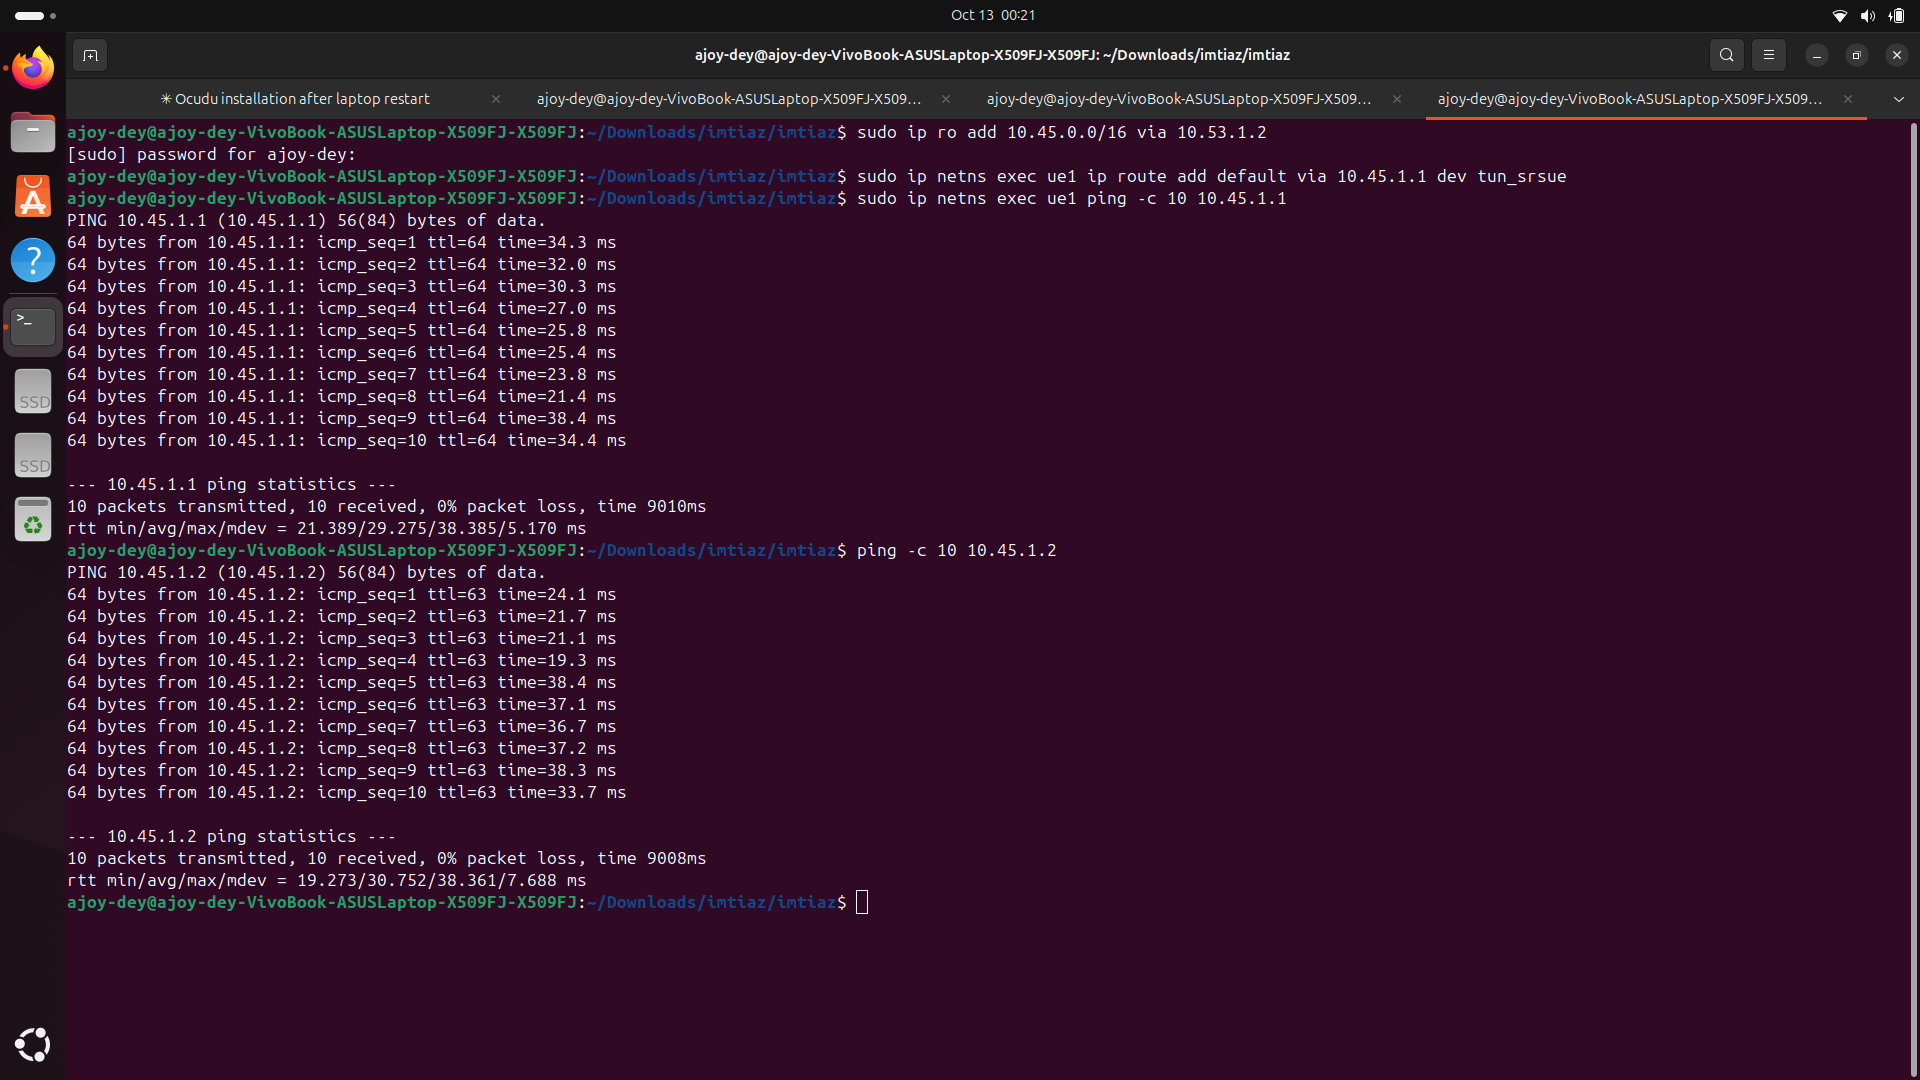
\includegraphics[width=0.95\textwidth]{ping_ul_dl.png}
\caption{Uplink and downlink ping through the 5G network: 0\% packet loss in both directions.}
\label{fig:ping}
\end{figure}

\subsection{gNB Live Metrics}

The gNB console metrics (\texttt{t} command) were captured while the UE was
idle and then under continuous load
(\texttt{ping -s 1000 -i 0.1 10.45.1.1}, i.e.\ 1000-byte packets every
100\,ms).

\begin{table}[H]
\centering
\begin{tabular}{l c c}
\toprule
Metric & Downlink & Uplink \\
\midrule
CQI / rank indicator   & 15 / 1 & -- / 1 \\
MCS                    & 28 & 6--7 \\
Bitrate (\texttt{brate}) & 100--112 kbps & 189--210 kbps \\
HARQ ACK / NACK per period & 20--24 / 0 & 60--66 / 0--1 \\
Block error rate       & 0\% & 0--1\% \\
PUSCH SINR             & -- & 2.8--2.9 dB \\
Timing advance         & -- & 518 ns \\
\bottomrule
\end{tabular}
\caption{gNB metrics under continuous ping load (RNTI 0x4601, PCI 1).}
\end{table}

\begin{figure}[H]
\centering
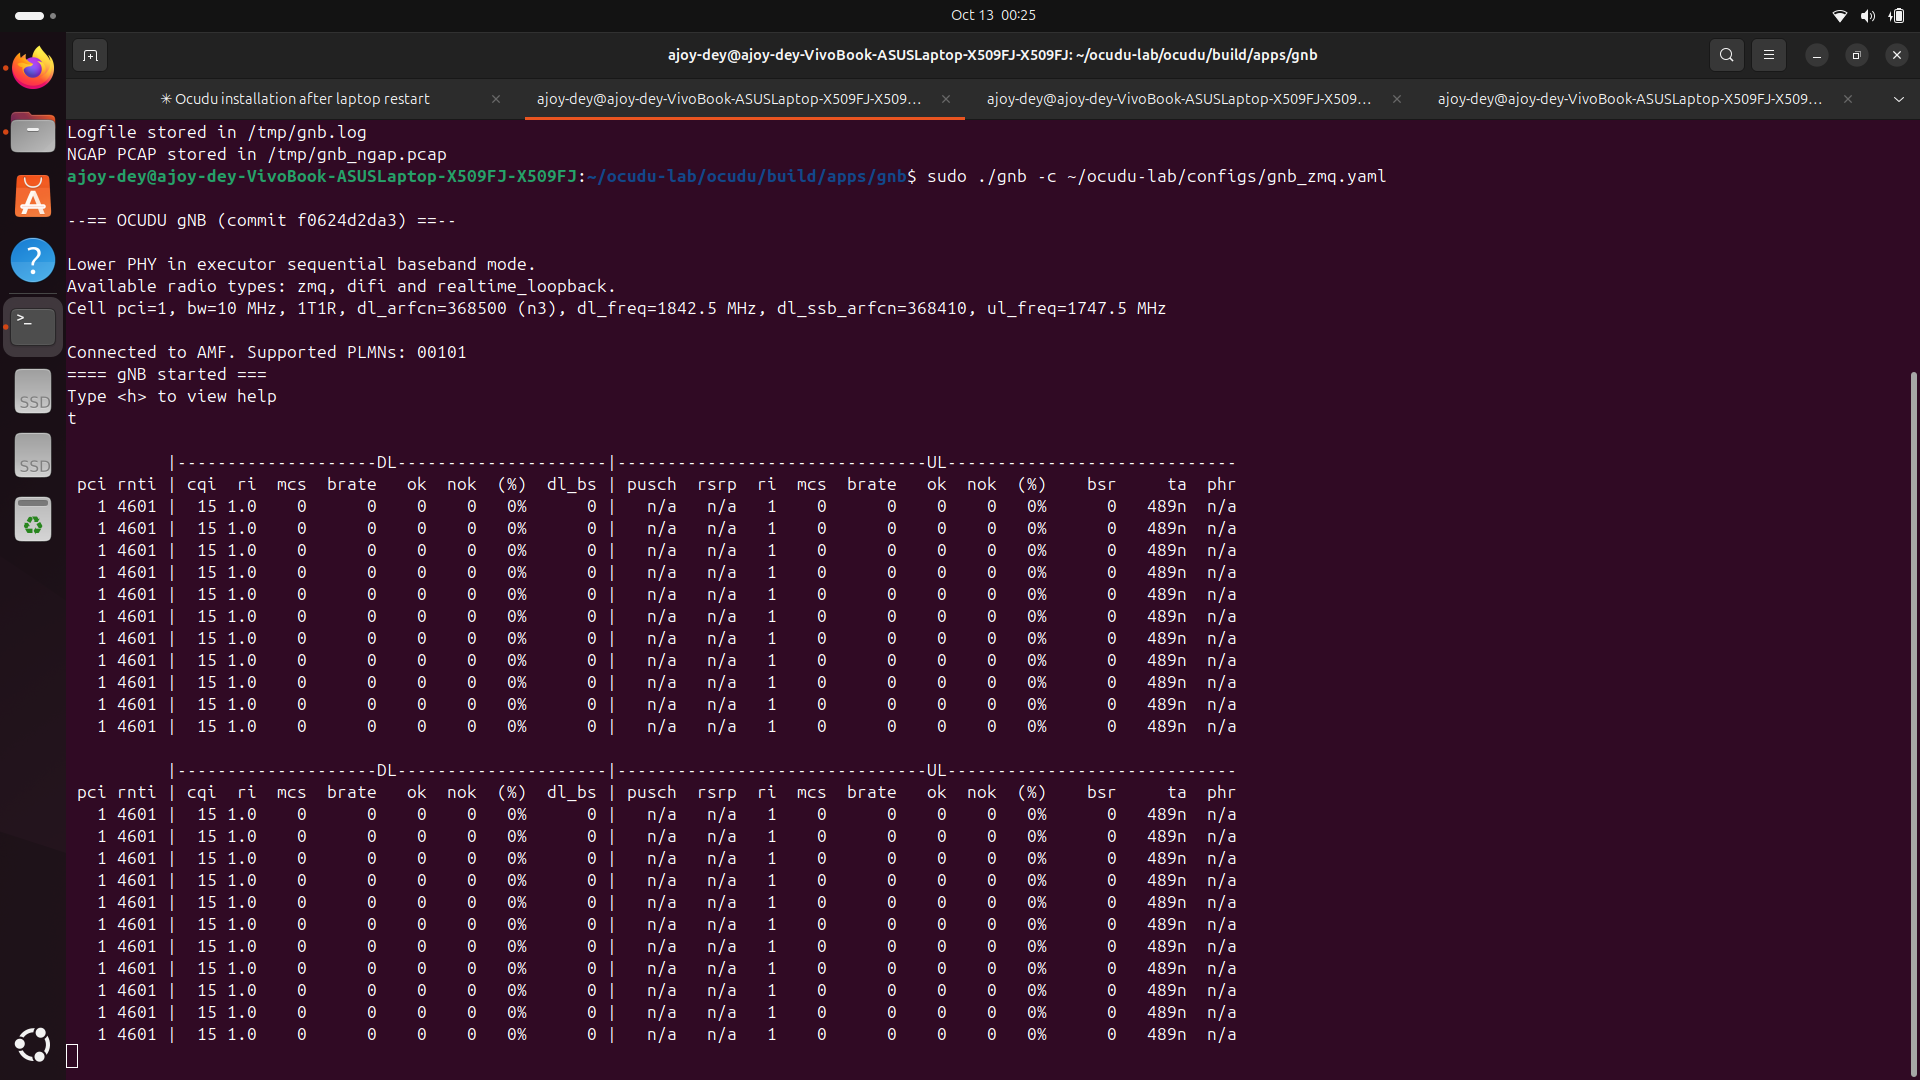
\includegraphics[width=0.95\textwidth]{gnb_metrics_idle.png}
\caption{gNB console after start-up: connected to the AMF, UE (RNTI 4601) attached and idle (CQI 15, no traffic).}
\label{fig:idle}
\end{figure}

\begin{figure}[H]
\centering
\begin{subfigure}{0.49\textwidth}
  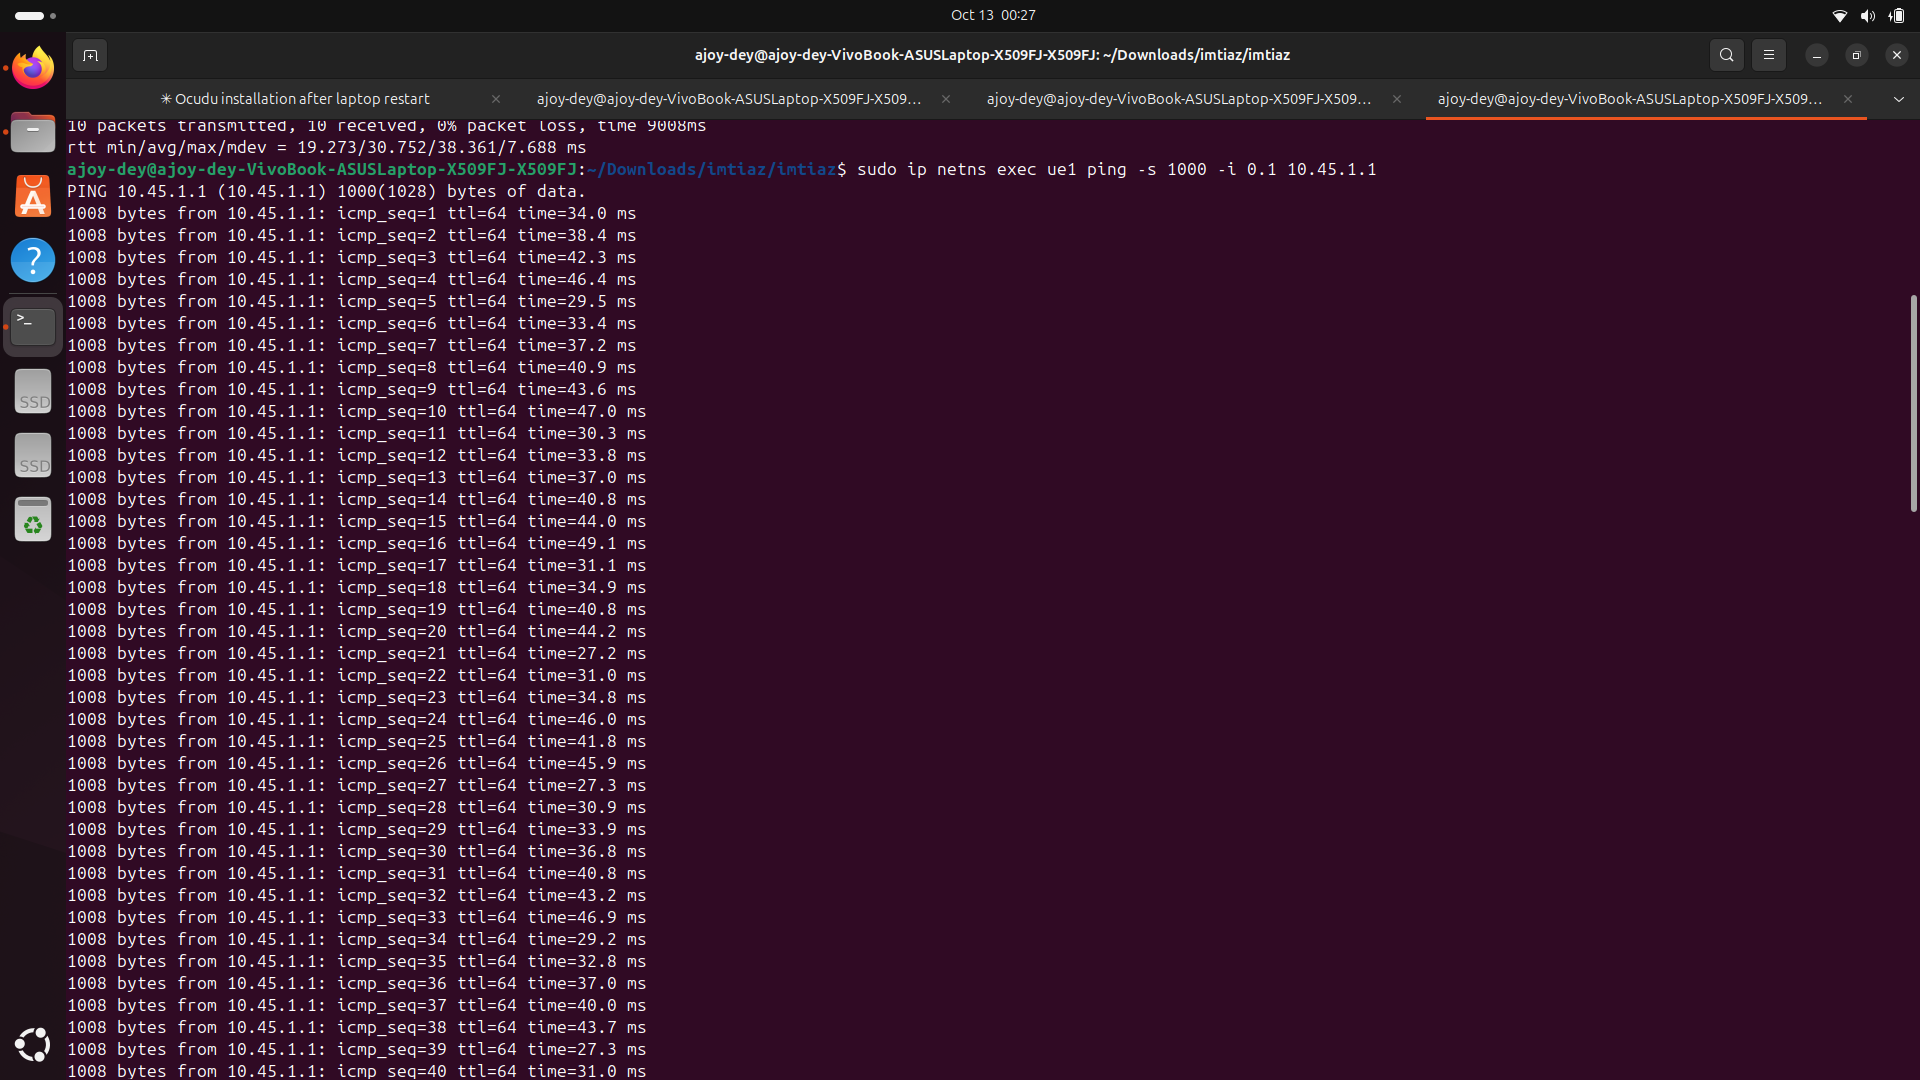
\includegraphics[width=\textwidth]{ping_continuous.png}
  \caption{Continuous 1000-byte ping from the UE.}
\end{subfigure}\hfill
\begin{subfigure}{0.49\textwidth}
  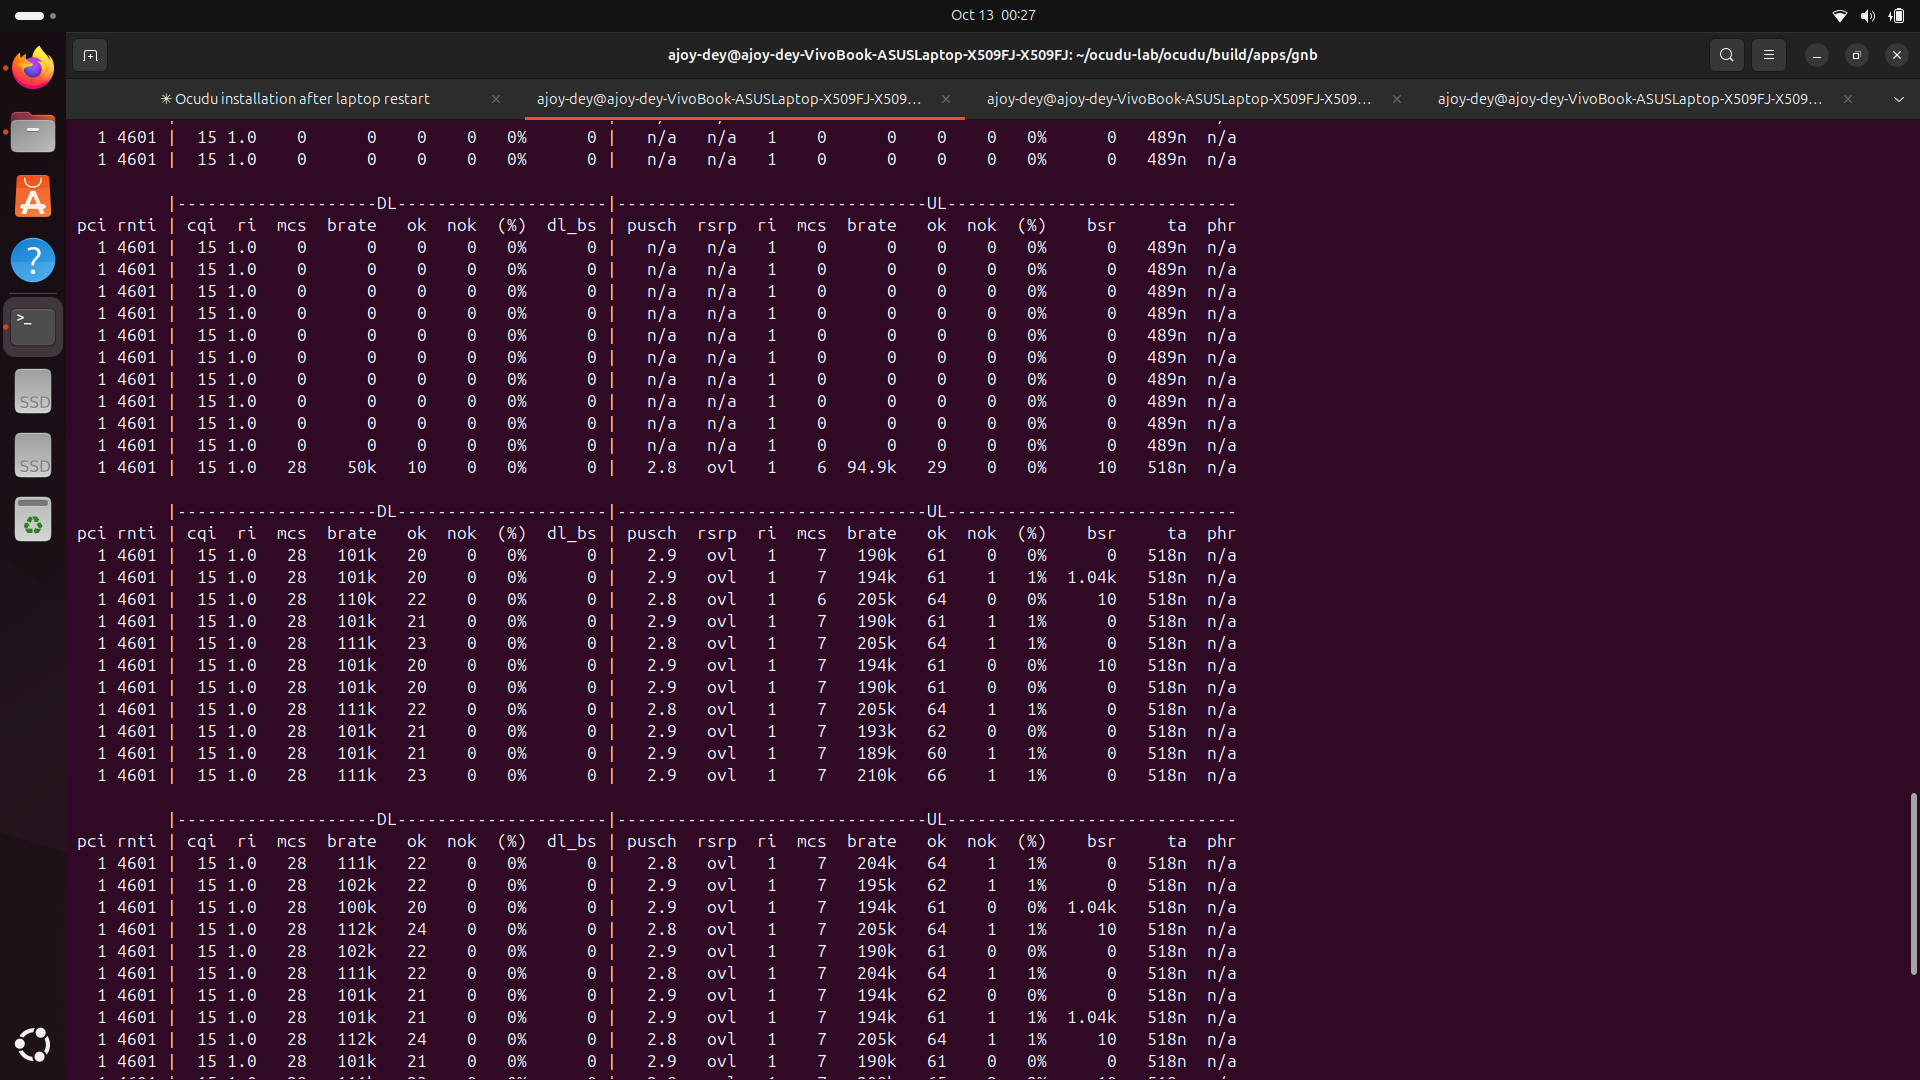
\includegraphics[width=\textwidth]{gnb_metrics_traffic.png}
  \caption{gNB metrics when traffic starts.}
\end{subfigure}
\caption{Traffic test. The metrics change from all-zero to active DL/UL
scheduling as soon as the ping starts.}
\label{fig:traffic}
\end{figure}

\subsubsection*{Observation: uplink saturation}
The uplink shows \texttt{rsrp = ovl} (overload) and a low PUSCH SINR of about
2.8\,dB, so the scheduler uses a low uplink MCS (6--7) while the downlink reaches
MCS 28. The likely cause is the UE transmit gain (\texttt{tx\_gain = 50} in
\fpath{ue\_zmq.conf}): with a lossless ZMQ link this amplitude clips the samples
received by the gNB. This does not affect the correctness of the test, and
uplink errors stay at 0--1\%. Reducing the UE \texttt{tx\_gain} should improve
uplink SINR and MCS; this has not been tested yet.

% ---------------------------------------------------------------------------
\section{Problems Encountered and Solutions}

\subsection{Problem 1: Laptop Freeze During Compilation}
\label{sec:p1}

\paragraph{Symptom.} About 14 minutes into the first build, the desktop turned
into a white, unresponsive screen. The laptop had to be restarted. The build
stopped at 37\%, and two object files were left empty (0 bytes).

\paragraph{Root cause.} The first attempt used \texttt{make -j8} while the
Open5GS Docker image was being built at the same time. OCUDU's ASN.1 sources
are large, and each Clang process can use 1--2\,GB of RAM, so eight parallel
compilers plus the Docker build exceeded the 11\,GiB of RAM. The system then
thrashed swap and the graphical session stopped responding. The kernel log
also showed a PCIe error from the Realtek RTL8821CE Wi-Fi driver
(\texttt{rtw88\_8821ce}) at 19:06:37, six minutes before the hang:
\begin{lstlisting}
rtw88_8821ce 0000:04:00.0: failed to dequeue 184 skb TX queue 1
pcieport 0000:00:1d.1: DPC: containment event, status:0x1f01:
    unmasked uncorrectable error detected
WARNING: ... rtw_dbi_read8.constprop.0+0xba/0xe0 [rtw88_pci]
\end{lstlisting}

\paragraph{Solution.}
\begin{enumerate}[itemsep=2pt]
  \item The two empty object files
        (\fpath{e2sm\_ccc.cpp.o}, \fpath{nrppa/common.cpp.o}) were moved out of
        the build tree so that \texttt{make} would rebuild them.
  \item The build was resumed incrementally (not from scratch) with 3 jobs,
        inside a \texttt{systemd} scope limited to 6\,GB of memory and 5 CPU
        cores, at the lowest CPU and I/O priority.
  \item The large jobs (OCUDU, tests, srsUE, Docker image) were run strictly
        one after another.
\end{enumerate}
Memory use then stayed at about 3.7--4.0\,GB with no swap usage, and the
desktop remained responsive for the whole build.

\subsection{Problem 2: UE Could Not Complete Registration}
\label{sec:p2}

\paragraph{Symptom.} The gNB connected to the AMF, and the UE completed RRC
setup, authentication and security mode. Then the gNB released the UE after
3\,s:
\begin{lstlisting}
[NGAP] UE did not request a PDU session after 3000ms. Requesting UE release
\end{lstlisting}

\paragraph{Root cause.} The srsUE log showed that it could not decode the NAS
Registration Accept message:
\begin{lstlisting}
[ASN1 ] [E] Decoding Failed (5GS tracking area identity list):
            Length (19) does not equal expected length 7
[NAS5G] [E] Unable to unpack complete NAS pdu
\end{lstlisting}
The AMF section of \fpath{ocudu/docker/open5gs/open5gs-5gc.yml} listed three
Tracking Area Codes (7, 8 and 9). A file comment says TACs 8 and 9 exist only
for a multi-TAC NTN example. With three TACs, the 5GS TAI list information
element is 19 bytes long, but srsUE's NAS decoder only accepts the 7-byte form
with a single TAC. Because the UE never processed the Registration Accept, it
never sent a PDU Session Establishment Request.

\paragraph{Solution.} TACs 8 and 9 were commented out in the AMF
configuration, leaving only TAC 7 (which matches the gNB). The Docker image
was rebuilt and the core restarted:
\begin{lstlisting}
  tai:
    - plmn_id:
        mcc: ${MCC}
        mnc: ${MNC}
      tac: 7
#    - plmn_id:   ... tac: 8   (disabled)
#    - plmn_id:   ... tac: 9   (disabled)
\end{lstlisting}
The original file is kept as \fpath{report/open5gs-5gc.yml.orig}. After the gNB
and UE were restarted, registration and PDU session establishment succeeded
immediately.

\paragraph{Note.} This change has to be reapplied if the OCUDU repository is
updated and the file is reset.

% ---------------------------------------------------------------------------
\section{Timeline}

\begin{table}[H]
\centering
\begin{tabular}{l l}
\toprule
Time (local, UTC+6) & Event \\
\midrule
12 Oct 18:54 & OCUDU and srsRAN\_4G cloned \\
12 Oct 18:58 & OCUDU CMake configured, first build started (\texttt{-j8}) \\
12 Oct 19:03 & Open5GS Docker build started in parallel \\
12 Oct 19:06 & Wi-Fi driver PCIe error in kernel log \\
12 Oct 19:12 & System hang at 37\% (Problem 1) \\
12 Oct 22:52 & Laptop restarted, diagnosis \\
12 Oct 22:59 & Build resumed with resource limits \\
12 Oct 23:50 & OCUDU build complete \\
12 Oct 23:55 & Unit tests complete (10\,569/10\,569 passed) \\
13 Oct 00:05 & srsUE build complete \\
13 Oct 00:10 & Open5GS image built, core started at 00:11 \\
13 Oct 00:13 & gNB connected to AMF \\
13 Oct 00:14 & First UE attempt fails at Registration Accept (Problem 2) \\
13 Oct 00:16 & Core reconfigured with single TAC and restarted \\
13 Oct 00:17 & UE registered, PDU session IP 10.45.1.2 \\
13 Oct 00:21 & Uplink and downlink ping: 0\% loss \\
13 Oct 00:27 & Load test and gNB metrics captured \\
\bottomrule
\end{tabular}
\caption{Chronology of the work.}
\end{table}

% ---------------------------------------------------------------------------
\section{How to Reproduce the End-to-End Test}

Start the components in this order, each in its own terminal:
\begin{lstlisting}[language=bash]
# 1. Core
cd ~/ocudu-lab/ocudu/docker && docker compose up -d 5gc

# 2. gNB (wait for "Connected to AMF")
cd ~/ocudu-lab/ocudu/build/apps/gnb
sudo ./gnb -c ~/ocudu-lab/configs/gnb_zmq.yaml

# 3. UE (wait for "PDU Session Establishment successful")
sudo ip netns add ue1
cd ~/ocudu-lab/srsRAN_4G/build/srsue/src
sudo ./srsue ~/ocudu-lab/configs/ue_zmq.conf

# 4. Routes and traffic
sudo ip ro add 10.45.0.0/16 via 10.53.1.2
sudo ip netns exec ue1 ip route add default via 10.45.1.1 dev tun_srsue
sudo ip netns exec ue1 ping -c 10 10.45.1.1
ping -c 10 10.45.1.2
\end{lstlisting}
Stop in reverse order: UE (Ctrl+C), gNB (Ctrl+C), then
\texttt{docker compose down}.

% ---------------------------------------------------------------------------
\section{Conclusion}

The OCUDU 5G gNB was successfully built from source with ZeroMQ support on a
modest laptop (4-core i5, 11\,GiB RAM). All 10\,569 unit tests passed. A
complete 5G SA system (Open5GS core, OCUDU gNB and srsUE) was brought up on
one machine without radio hardware. The UE registered, obtained IP address
10.45.1.2, and exchanged traffic in both directions with 0\% packet loss and
about 30\,ms average round-trip time. The gNB reported CQI 15 and downlink
MCS 28.

Two lessons are useful for future work: (i) on machines with limited RAM, the
OCUDU build must run with reduced parallelism and memory limits; and (ii) when
srsUE is used with the OCUDU Docker core, the AMF must advertise a single TAC.

\subsection*{Possible Next Steps}
\begin{itemize}[itemsep=2pt]
  \item Tune the UE \texttt{tx\_gain} to remove uplink overload and measure the
        resulting uplink MCS and throughput.
  \item Measure throughput with \texttt{iperf3} in both directions.
  \item Analyse the captured NGAP/MAC/NAS PCAP files
        (\fpath{runtime/gnb\_ngap.pcap}, \fpath{runtime/ue\_nas.pcap}) in Wireshark.
  \item Try multiple UEs, the split CU/DU deployment, or a real SDR
        (USRP with UHD) and a low-latency kernel.
\end{itemize}

% ---------------------------------------------------------------------------
\appendix
\section{Configuration Files}

\subsection{gNB: \texttt{gnb\_zmq.yaml} (main parameters)}
\begin{lstlisting}
cu_cp:
  amf:
    addr: 10.53.1.2
    port: 38412
    bind_addr: 10.53.1.1
    supported_tracking_areas:
      - tac: 7
        plmn_list:
          - plmn: "00101"
            tai_slice_support_list:
              - sst: 1
  inactivity_timer: 7200
ru_sdr:
  device_driver: zmq
  device_args: tx_port=tcp://127.0.0.1:2000,rx_port=tcp://127.0.0.1:2001,base_srate=11.52e6
  srate: 11.52
  tx_gain: 0
  rx_gain: 0
cell_cfg:
  dl_arfcn: 368500
  band: 3
  channel_bandwidth_MHz: 10
  common_scs: 15
  plmn: "00101"
  tac: 7
  pdcch:
    common:
      ss0_index: 0
      coreset0_index: 6
    dedicated:
      ss2_type: common
      dci_format_0_1_and_1_1: false
  prach:
    prach_config_index: 1
    total_nof_ra_preambles: 64
    nof_ssb_per_ro: 1
    nof_cb_preambles_per_ssb: 64
  pdsch:
    mcs_table: qam64
  pusch:
    mcs_table: qam64
\end{lstlisting}

\subsection{UE: \texttt{ue\_zmq.conf}}
\begin{lstlisting}
[rf]
freq_offset = 0
tx_gain = 50
rx_gain = 40
srate = 11.52e6
nof_antennas = 1
device_name = zmq
device_args = tx_port=tcp://127.0.0.1:2001,rx_port=tcp://127.0.0.1:2000,base_srate=11.52e6

[rat.eutra]
dl_earfcn = 2850
nof_carriers = 0

[rat.nr]
bands = 3
nof_carriers = 1
max_nof_prb = 52
nof_prb = 52

[usim]
mode = soft
algo = milenage
opc  = 63BFA50EE6523365FF14C1F45F88737D
k    = 00112233445566778899aabbccddeeff
imsi = 001010123456780
imei = 353490069873319

[rrc]
release = 15
ue_category = 4

[nas]
apn = internet
apn_protocol = ipv4

[gw]
netns = ue1
ip_devname = tun_srsue
ip_netmask = 255.255.255.0
\end{lstlisting}

\subsection{Core subscriber entry (\texttt{open5gs.env})}
\begin{lstlisting}
SUBSCRIBER_DB=001010123456780,00112233445566778899aabbccddeeff,opc,
              63bfa50ee6523365ff14c1f45f88737d,8000,9,10.45.1.2
\end{lstlisting}

\section{Evidence Files}

All files are in \fpath{\textasciitilde/ocudu-lab/report/}:
\begin{itemize}[itemsep=1pt]
  \item \fpath{cmake\_ocudu.log}, \fpath{make\_ocudu.log}, \fpath{make\_ocudu\_resume.log}: OCUDU configuration and build
  \item \fpath{make\_test\_ocudu.log}: unit test results
  \item \fpath{cmake\_srsran.log}, \fpath{make\_srsran.log}: srsUE build
  \item \fpath{docker\_build\_5gc.log}, \fpath{docker\_rebuild\_5gc.log}: core image builds
  \item \fpath{open5gs-5gc.yml.orig}: original AMF configuration (before the TAC fix)
  \item \fpath{ping\_ul\_dl.png}, \fpath{ping\_continuous.png}, \fpath{gnb\_metrics\_idle.png}, \fpath{gnb\_metrics\_traffic.png}: screenshots
  \item Runtime logs and captures: \fpath{runtime/gnb.log}, \fpath{runtime/ue.log}, \fpath{runtime/*.pcap} (copied from \fpath{/tmp})
\end{itemize}

\end{document}
